To measure memory read latency we read the first byte of each cache line within a span of memory.  
We measure the time taken per read and then compute the mean and standard deviation of the time by span size.
As the span size increases, the depth of memory reached goes from L1 to L2 and finally to main memory.  
Larger spans would eventually reach to the secondary storage due to paging but very large spans would be needed and thus paging is measured in a later experiment.

The reading code follows this pseudo code pattern:
\begin{verbatim}
for(k = 0; k < 2^SPAN_SIZE; k+= PAGE_SIZE){
	x = data[k];
}
\end{verbatim}

Documentation shows that the L1 cache has a 3 cycle load-to-use delay.  Since we are just reading into a register allocated variable we thus expect a 3 cycle delay over the baseline measurement.  No data on the load-to-use delay of the L2 or the main memory can be found.  A stack overflow article comparing speeds of typical caches state that L2 is typically 10x slower than L1 and main memory is typically 200x slower.  Thus we expect 14 cycles for L1 access, 41 for L2, and 600 for main memory.

In figure \ref{fig:exp_2_1} we see that the L1 cache latency is about 26 cycles, L2 about 70 cycles, and main memory about 150 cycles.  We believe there may be extra overhead in our measurements that we are failing to account for in L1/L2 memory (possibly x isn't being put into a register or similar) we will investigate this further.  Main memory is significantly faster than prediction, our guess is that this is related to the main memory of the rasberry pi being on chip and thus faster than typical latencies. We will attempt to find better documentation for our final report.  We also believe that there may be out of order execution causing pipelining of reading,  we are looking for ways to improve our timing code.

\begin{figure}[h]
\label{fig:exp_2_1}
\centering
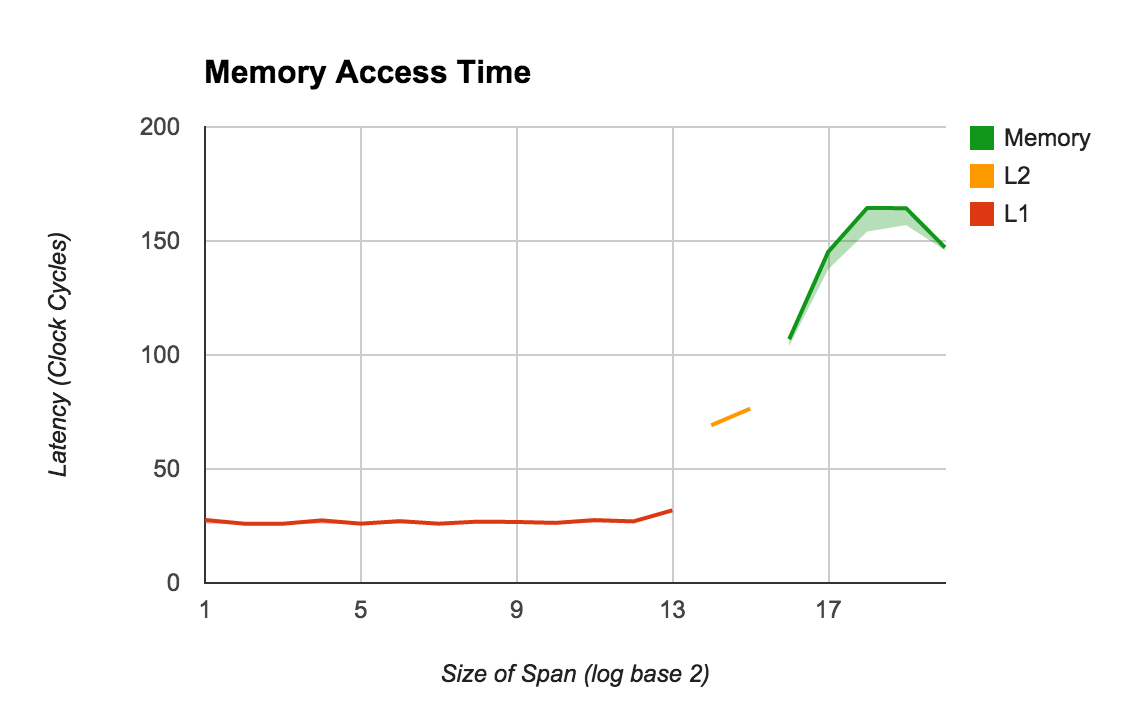
\includegraphics[scale=.5]{experiments/exp_2_1_fig.png}
\caption{Cycle count for memory read latency vs span size.  
Different memory regimes are labeled by color.  +/- 1 standard deviation highlighted by shading.}
\end{figure}